\documentclass{article}
\setlength\parindent{24pt}
\usepackage[margin=0.6in]{geometry}
\usepackage{indentfirst}
\usepackage{amsmath}
\usepackage{graphicx}
\usepackage{float}
\usepackage[utf8]{inputenc}
\usepackage{listings}
\usepackage{color}
\usepackage{enumerate}
\usepackage[portuguese]{babel}

\definecolor{dkgreen}{rgb}{0,0.6,0}
\definecolor{gray}{rgb}{0.5,0.5,0.5}
\definecolor{mauve}{rgb}{0.58,0,0.82}

\lstset{frame=tb,
  language=Matlab,
  aboveskip=3mm,
  belowskip=3mm,
  showstringspaces=false,
  columns=flexible,
  basicstyle={\small\ttfamily},
  numbers=none,
  numberstyle=\tiny\color{gray},
  keywordstyle=\color{blue},
  commentstyle=\color{dkgreen},
  stringstyle=\color{mauve},
  breaklines=true,
  breakatwhitespace=true,
  tabsize=4
}

\renewcommand{\baselinestretch}{1.0}

\begin{document}

\title{EA614 - Análise de Sinais \\
\large{EFC3 - Série de Fourier}}
\author{Rafael Gonçalves (186062)}
\date{\today}

\maketitle

\section{Parte Computacional}

\begin{enumerate}[(a)]
    \item
No caso de $x(t)$ temos:

\begin{equation}
a_{k} = \frac{1}{T}\int_{\frac{-T}{2}}^{\frac{T}{2}}x(t)e^{-jk\omega_{0}t}dt = \frac{1}{T}\int_{\frac{-T}{2}}^{\frac{T}{2}}\frac{2}{T}te^{-jk\omega_{0}t}dt
\end{equation}

$T = 4s$ então podemos escrever como:

\begin{equation}
    a_k = \frac{2}{T^{2}}\int_{-2}^{2}te^{-jk\omega_{0}t}dt
\end{equation}

Para $k = 0$ (nível DC):

\begin{equation}
    a_0 = \frac{2}{T^{2}}\int_{-2}^{2}te^{0}dt = \frac{2}{T^{2}}\int_{-2}^{2}tdt 
\end{equation}

\[
    \boxed{a_0 = 0}
\]

Para $k \neq 0$ podemos resolver a integração por partes:

\begin{center}
    $\int u dv = u v - \int v du$\break

    $u = t ; \quad  du = dt$\break

   $v = \frac{-e^{jk\omega_0t}}{jk\omega_0}; \quad dv = e^{jk\omega_0t}dt$
\end{center}
Então:

\begin{equation}
    \int te^{-jk\omega_{0}t}dt = -t \frac{e^{jk\omega_0t}}{jk\omega_0} + \int \frac{e^{jk\omega_0t}}{jk\omega_0} dt 
\end{equation}

\begin{equation}
    a_k = \frac{2}{T^2} \left ( \left [ - t\frac{e^{jk\omega_0t}}{jk\omega_0} \right ]_{-2}^2 + \int_{-2}^2 \frac{e^{jk\omega_0t}}{jk\omega_0}dt \right )= \frac{2}{T^2} \left [ \frac{e^{jk\omega_0t}}{jk\omega_0} \left ( t + \frac{1}{jk\omega_0} \right ) \right ] _{-2}^2
\end{equation}

\begin{equation}
    a_k = \frac{2}{T^2} \left [ \frac{-2}{jk\omega_0} \left ( e^{jk\omega_0 2} + e^{-jk\omega_0 2} \right ) + \frac{-1}{k^2 \omega_0 ^2} \left ( e^{jk\omega_0 2} - e^{-jk\omega_0 2} \right ) \right ]
\end{equation}


Usando a fórmula de Euler temos:

\begin{center}
    $\omega_0 = \frac{2\pi}{T}$ e $T = 4s$
\end{center}

\begin{equation}
    a_k = \frac{2}{4^2} \left [ \frac{-4 \cdot 2}{jk\pi}\cos(\pi k) - \frac{4j}{k^2 \pi^2}\sin(\pi k) \right ]
\end{equation}

\[
    \boxed{a_k = \frac{j}{k \pi} \cos(k \pi)}
\]

\break\vfill

\item
A função implementada (plot\_fourier) retorna a aproximação por série de fourier (dado número de aproximações N, coeficientes a, intervalo de tempo t e frequência w0). Além disso a mesma função será usada no próximo item para plotar os gráficos da aproximação por meio da variável de controle (plot\_var = 1).

\begin{lstlisting}
t = -2:0.0001:2;
T = 4;
a = @(k) (i*cos(k*pi))/(k*pi);
w0 = 2*pi/T;

function X = plot_fourier(N, a, t, w0, plot_var),
    X = zeros(size(t));
    for k = 1:N,
        X = X + a(k)*exp(i*k*w0*t);
        X = X + a(-k)*exp(i*(-k)*w0*t);
    end;
    if plot_var == 1,
        plot(t, X)
        xlabel ("t");
        title (["Serie de Fourier com ", num2str(N), " termos"]);
    end;
end;
\end{lstlisting}

\item

 Gráficos com a função dente de serra e as aproximações (respectivamente N = 1, 10, 20 e 50).

 \begin{figure}[h!]
 \centering
 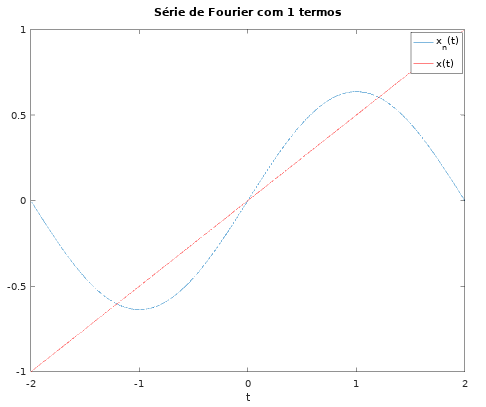
\includegraphics[width=0.5\textwidth]{images/plot_n1.png}
     \caption{Aproximação por série de Fourier com N = 1}
 \end{figure}

 \begin{figure}[h!]
 \centering
 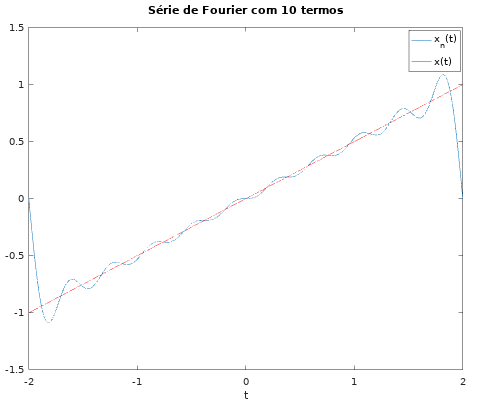
\includegraphics[width=0.5\textwidth]{images/plot_n10.png}
     \caption{Aproximação por série de Fourier com N = 10}
 \end{figure}

 \begin{figure}[h!]
 \centering
 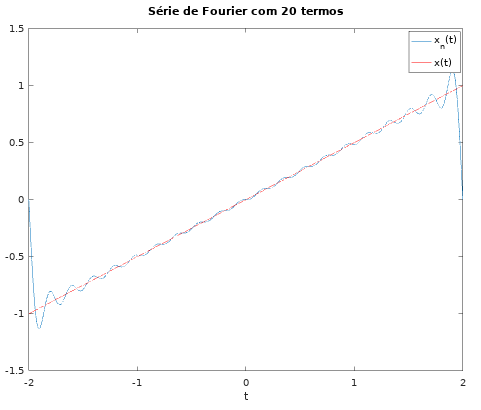
\includegraphics[width=0.5\textwidth]{images/plot_n20.png}
     \caption{Aproximação por série de Fourier com N = 20}
 \end{figure}

 \begin{figure}[h!]
 \centering
 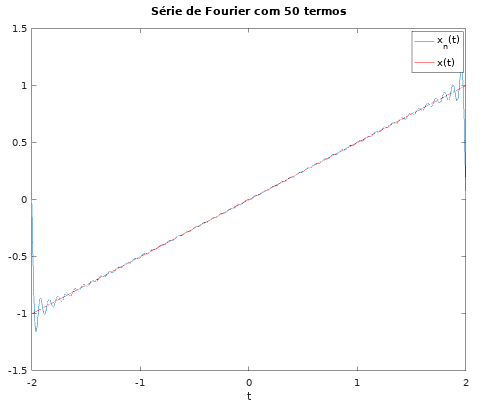
\includegraphics[width=0.5\textwidth]{images/plot_n50.png}
     \caption{Aproximação por série de Fourier com N = 50}
 \end{figure}

\break
\vspace*{\fill}
\break

\item 
    Os erros $\left ( \frac{\sum\limits _{k = -N} ^{N} (x(t) - x_N(t))^2}{2N+1} \right )$ encontrados pelo programa para $E_N$ onde N é o número do último termo da série de fourier (ou seja, série de fourier calculada para $-N \leq k \leq N$):
\hfill\break

$E_1 = 0.13071$

$E_{10} = 0.019309$

$E_{20} = 0.0099078$

$E_{50} = 0.0040375$

\break\hfill

\item

Gráfico do módulo dos coeficientes $a_k$ em função de $\omega = 2 \pi k$:

\begin{figure}[H]
\centering
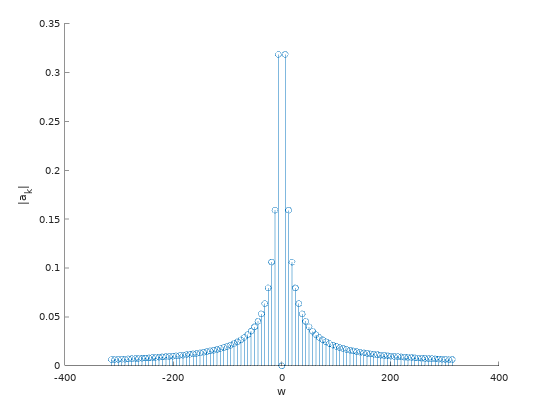
\includegraphics[width=0.5\textwidth]{images/ak_x_w.png}
    \caption{Gráfico do módulo de $a_k$ por $\omega$}
\end{figure}

\item

Sendo:

\begin{equation}
    \omega_C = \frac{1}{RC} = 10 \frac{rad}{s}
\end{equation}

\begin{equation}
    H(j \omega) = \frac{1}{1 - \left ( \frac{\omega_C}{\omega} \right )}
\end{equation}

Temos que a resposta em frequência é dada graficamente por:

\begin{figure}[H]
\centering
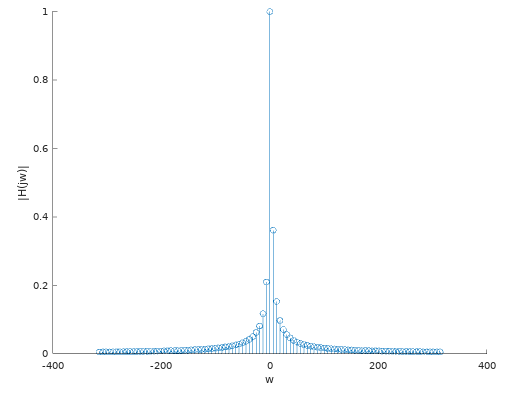
\includegraphics[width=0.5\textwidth]{images/abs_x_w.png}
    \caption{Gráfico do módulo de $H(j\omega)$ por $\omega$}
\end{figure}

\begin{figure}[H]
\centering
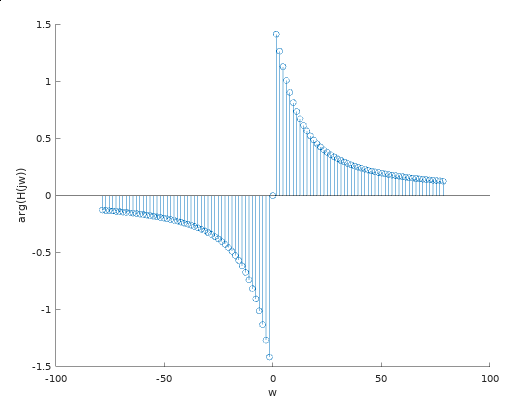
\includegraphics[width=0.5\textwidth]{images/arg_x_w.png}
    \caption{Gráfico da fase de $H(j\omega)$ por $\omega$}
\end{figure}

O gráfico plotado é um filtro passa alta (como visto no gráfico do modulo, o ganho é maior para frequências maiores).

\item
Gráfico da saída $y(t)$ quando $x(t)$ é o sinal dente de serra:
\begin{figure}[H]
\centering
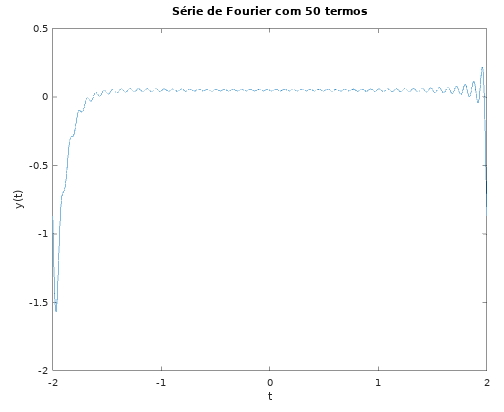
\includegraphics[width=0.5\textwidth]{images/y.png}
    \caption{Gráfico da resposta do sinal $x(t)$ após passar pelo filtro RC}
\end{figure}
    Só passaram as frequências mais altas e portanto o sinal ficou achatado no centro (majoritariamente próximo ao zero, pois os termos de frequência menor são responsáveis pela forma "macro" do sinal) enquanto que o sinal todo continua apresentando os "ruídos" causados pelos termos de alta frequência (percebidos sobretudo nas bordas).


\end{enumerate}
\end{document}
